\documentclass[11pt]{article}

\usepackage{mtsxiv}
%\usepackage{url}
\usepackage[colorlinks=true,citecolor=black,linkcolor=black,urlcolor=blue]{hyperref}
%\usepackage{times}
\usepackage{multirow}
\setlength\titlebox{6.5cm}    % Expanding the titlebox



\usepackage{polyglossia}
\setdefaultlanguage[variant=australian]{english}
\usepackage{latexsym}
%\usepackage[small,bf]{caption}
\usepackage[bf]{caption}
\usepackage{xltxtra}
\usepackage{times}
\usepackage{fontspec}
\defaultfontfeatures{PunctuationSpace=3,Scale=MatchLowercase,Mapping=tex-text}
\newfontfeature{IPA}{+mgrk}
%\setromanfont[IPA]{FreeSerif}
\setromanfont[Scale=0.9]{Times New Roman}
\newfontfamily\qipa[IPA,Scale=MatchLowercase]{FreeSerif}
\newfontfamily\qipb[IPA,Scale=MatchLowercase]{Junicode}
\setmonofont[Scale=0.7]{DejaVu Sans Mono}
\newfontfamily\smallertt[Scale=0.55]{DejaVu Sans Mono}
\newfontfamily\smallerrm[Scale=0.85]{Times New Roman}

%\fontspec[FakeBold=2.5]{Times New Roman}
%\DeclareFontShape{EU1}{TimesNewRoman(0)}{m}{sc}{<->ssub * TimesNewRoman(1)/m/sc}{}

\newcommand{\email}[1]{\texttt{\href{mailto:#1}{#1}}}
\usepackage{natbib}
%\usepackage{natbib,natbibspacing}
\usepackage{setspace}
\usepackage{booktabs}

\usepackage{gb4e}  % for numbered examples
\usepackage{expex} % another possibility

%\usepackage{subfigure}
%\usepackage{subfloat}
\usepackage{subfig}

%\setlength{\bibspacing}{\baselineskip-0.4em}

\newenvironment{itemise}[1]{
        \begin{itemize}\setlength{\itemsep}{-0.3em}
		  %\setlength{\itemindent}{-1em}
		  %\setlength{\leftmargin}{-2em}
        \vspace{-0.6em}
        #1
}{
        \end{itemize}
        \vspace{-1pt}
}

\newcommand{\todo}[1]{\{\textbf{TODO: #1}\}}


%\setlength\titlebox{6.5cm}    % You can expand the title box if you
% really have to

\newcommand{\tag}[1]{{\small{\texttt{#1}}}}
\newcommand{\gmk}[1]{{\qipb\scshape #1}}
\newcommand{\eng}[1]{`#1'}

%%\Keywords{Kazakh, Tatar, MT, Free software, Open-source}

\newcommand{\confname}{Machine Translation Summit XIV}
\newcommand{\website}{\protect\url{http://www.mtsummit2013.info/}}
\newcommand{\contactname}{research track co-chair Mikel L.\ Forcada}
\newcommand{\contactemail}{mlf@dlsi.ua.es} 
\newcommand{\conffilename}{mtsxiv}
\newcommand{\downloadsite}{\protect\url{http://www.mtsummit2013.info/}}
\newcommand{\paperlength}{$8$ (eight)}
\newcommand{\shortpaperlength}{$4$ (four)}

\title{A free/open-source Kazakh-Tatar machine translation system}

\author{Ilnar Salimzyanov\\
  Kazan Federal University\\
  Kazan, Republic of Tatarstan\\
  Russian Federation\\
  \email{ilnar.salimzyan@gmail.com}  \And
  Jonathan North Washington\\
  Departments of Linguistics\\
  and Central Eurasian Studies\\
  Indiana University\\
  Bloomington, Indiana 47405 USA\\
  \email{jonwashi@indiana.edu}  \And
  Francis Morton Tyers\\
  Departament de Llenguatges\\
  i Sistemes Informàtics\\
  Universitat d'Alacant\\
  E-03877 Alacant\\
  \email{ftyers@dlsi.ua.es}}

\date{\today}






\begin{document}
\spacing{1}
\maketitle
\begin{abstract}
This paper presents a bidirectional machine translation system between Kazakh and Tatar.
\todo{expand abstract}
\end{abstract}
%FIXME
%\maketitleabstract

\section{Introduction}

This paper presents a prototype shallow-transfer rule-based machine translation
system between Kazakh and Tatar.

The paper will be laid out as follows: Section~\ref{sec:lang}\ gives a brief
description of the two languages; Section~\ref{sec:prev}\ gives a short review
of some previous work in the area of Turkic--Turkic language translation;
Section~\ref{sec:sys}\ describes the system and the tools used to construct it;
Section~\ref{sec:eval}\ gives a preliminary evaluation of the system; and
finally Section~\ref{sec:conc}\ describes our aims for future work and some
concluding remarks.

\section{Previous work}
\label{sec:prev}

Within the Apertium project, work on MT systems between Turkic languages has been started (Turkish--Kyrgyz, Azeri--Turkish, Turkish-Bashkir), but the Kazakh--Tatar system described by the present study is the closest to production-ready of them.  Among these systems is a prototype Tatar-Bashkir machine translation system which was built by the authors of this paper \citep{tyerswashingtonsalimzyanbattalov12}; due to the closeness of these languages, it proved to provide high accuracy in its translations, but being a prototype system by design, had relatively low coverage.

Besides these systems, several previous works on making machine translation systems between Turkic languages 
exist, although to our knowledge none are publically available.
Some MT systems have been reported that translate between Turkish and other Turkic languages, 
including Turkish--Crimean Tatar \citep{altintas01},
Turkish--Azerbaijani \citep{hamzaoglu93}, Turkish--Tatar \citep{suleymanov08}, and
Turkish--Turkmen \citep{tantug07}, though none of these have been released to a public audience. The Turkish--Azerbaijani
pair is also available through Google Translate.\footnote{\url{http://translate.google.com}}

%FIXME: mention tr-az, tr-ky?

%maybe this should be moved to 'Future plans'
%Within the Apertium project, work on several Turkic-language MT systems has been started, with the ultimate goal of creating independent but compatible
%finite-state transducers for each language.
%% The idea is that we started Kazakh-Tatar pair to be able to take into account
%% characteristics of two more distant Turkic languages, avoiding narrowing
%% ourselves to mutually intellegible Tatar and Bashkir, but generate
%% transducers which are still compatible and very coherent. Bashkir part of the
%% pair will be updated to the latest developments of Tatar transducer, which
%% took place while working on Kazakh-Tatar.

\section{Languages}
\label{sec:lang}

Both Tatar and Kazakh belong to the Kypchak (or Northwestern) group of Turkic
languages.  The spoken and written languages share some level of mutual intelligibility to native 
speakers, though this is somewhat limited, and is obscured by different orthographical 
conventions and some opaque correspondences.

Kazakh is primarily spoken in Kazakhstan, where it is the national
language, sharing official status with Russian as an official language.
Large groups of native speakers also exist in China, neighbouring
Central-Eurasian republics, and Mongolia. The total number of speakers is at least 10 million people.

Tatar is spoken in and around Tatarstan by
approximately 6 million people. It is co-official with Russian in Tatarstan ---
a republic within Russia.  A majority of native speakers of both languages are bilingual in Russian. %, and the standard varieties our system FIXMEs are written in Cyrillic.

%FIXME: Contrastive grammar
\subsection{Phonological differences}
%a generalised summary, 2 or 3 small specific examples
As closely related languages, Kazakh and Tatar share many phonological processes, including 
front-back vowel harmony systems, consonant voicing assimilation, and even a typologically rare 
consonantal nasal harmony system.  However, the differing details of these processes and the existence of 
processes unique to each language render Kazakh and Tatar fairly different.  For example, Kazakh has a 
ubiquitous system of desonorisation of the initial sonorants found in many common morphemes.  Furthermore, Tatar 
has nasal assimilation of the initial /l/ of the plural-suffix.

\subsection{Orthographic differences}
%a generalised summary, 1 or 2 small specific examples
The standard varieties of Kazakh and Tatar our system deals with are both written in Cyrillic, though their 
implementations of Cyrillic differ in many ways.

While Tatar and Kazakh both have a velar/uvular obstruent distinction (e.g., /k/ vs.\ /q/) that interacts with 
adjacent vowels, the Tatar orthography only has one series of letters (e.g., ‹к›), relying on adjacent 
vowels (and employing ъ `hard sign' and ь `soft sign' when these fail) to differentiate the two, and Kazakh 
has two series of obstruents (e.g., ‹к› and ‹қ›).

Kazakh does not orthographically distinguish high unrounded vowels (/{\qipa ɘ}/ ‹і› and /ə/ ‹ы›) before 
glides (/w/ ‹у› and /j/ ‹й›) by writing the combination with one letter; i.e., /{\qipa ɘ}j/ and /əj/ are both 
written ‹и›, while /{\qipa ɘ}w/ and /əw/ are both written ‹у›.  The quality of these vowels is necessary to know in 
order to predict the quality of following harmonising vowels. %, so this convention presents accute challenges to producing an accurate morphological transducer.
Additionally, Tatar and Kazakh both use `yoticised' vowels---i.e., when ‹о›, ‹у›, or ‹а› (along with ‹ә› in 
Tatar) follow /j/, a single character is used to represent both: ‹ё›, ‹ю›, and ‹я› respectively.\footnote{Furthermore, in Tatar, /j/ followed by ‹э› or ‹ы› in Tatar is represented by ‹е›, though ‹е› is also the non-word-initial variant of ‹э›.}  %Combined with the issues regarding ‹у› in Kazakh,

All of these orthographical conventions present acute challenges to designing accurate morphological transducers for the languages.

\subsection{Morphological differences}
There are a number of examples where the morphologies of Kazakh and Tatar are rather different, including 
morphemes in one language that do not exist in the other, entirely different uses of the same morpheme 
combinations, and morphotactic differences (i.e., allowable ordering and placement of morphemes).

An example of a morpheme that does not exist in one of the two languages is Kazakh -\texttt{\{E\}т\{I\}н}, 
which is used to form non-past verbal adjectives and verbal nouns.  The semantically equivalent structure 
in Tatar is -\texttt{\{E\} торган}, which historically corresponds to the source of the Kazakh morpheme; 
however, the use of -\texttt{\{E\} тұрған} in modern Kazakh is different from that of -\texttt{\{E\}т\{I\}н}.

%Another example of a far-reading morphological difference between Tatar and Kazakh reflects the presence of a four-way distinction in Kazakh's 2nd person system, where Tatar only has a two-way distinction.  Kazakh has a distinct pronoun for all combinations of [±plural, ±formal] (сен, сендер, сіз, сіздер), whereas Tatar collapse all pronouns except the [-plural, -formal] син into one pronoun (сез).  This does not only affect affect the pronoun system: since all finite verb forms morphologically agree in person and number with their subject and all possessed nouns agree in person and number with their possessor (with pronouns used in both circumstances only for emphasis and clarification, as is typical in pro-drop languages), the Kazakh and Tatar systems of agreement suffixes have the same pattern.
Another example of a far-reaching morphological difference between Tatar and Kazakh is the presence of a 
four-way distinction in Kazakh's 2nd person system (both pronouns and agreement suffixes), where Tatar only 
has a two-way distinction.  Kazakh has a distinct pronoun for all combinations of [±plural, ±formal], 
whereas Tatar collapses all pronouns except the [-plural, -formal] into one pronoun, as summarised in table~\ref{tab:2pprons}.
\begin{table}[htbp]
	\centering
%\begin{subtables}
	%\begin{subtable}[l]
	%\subtable[Kazakh 2nd person pronouns]{
	%\begin{subtable}
	\subfloat[Kazakh 2nd person pronouns]{
		\begin{tabular}{lll}
			\toprule
			 & {[$-$pl]} & {[$+$pl]} \\\midrule
			{[$-$formal]} & сен & сендер \\
			{[$+$formal]} & сіз & сіздер \\\bottomrule
		\end{tabular}
	%	\caption{Kazakh 2nd person pronouns}
	%\end{subtable}
	%\end{subtable}
	%\begin{subtable}
	%\begin{subtable}
	%}\subtable[Tatar 2nd person pronouns]{
	}\\
	\subfloat[Tatar 2nd person pronouns]{
		\begin{tabular}{lll}
			\toprule
			 & {[$-$pl]} & {[$+$pl]} \\\midrule
			{[$-$formal]} & син & сез \\
			{[$+$formal]} & сез & сез \\\bottomrule
		\end{tabular}%}
	%	\caption{Kazakh 2nd person pronouns}
	%\end{subtable}
	%\end{subtable}
	}
	\caption{The 2nd person pronoun systems of Kazakh and Tatar}
	\label{tab:2pprons}
\end{table}
%\end{subtables}

This systematic difference would seem to be a minor issue, since, as is typical in pro-drop languages, pronouns 
are only used for emphasis and clarification.  However, this difference between Tatar and Kazakh in 
the second-person system runs much deeper than just the pronoun system.  Since all finite verb forms 
morphologically agree in person and number with their subject and all possessed nouns agree in person and 
number with their possessor (even when there is no overt pronoun, in either situation), the Kazakh and Tatar 
systems of agreement suffixes reflect the same pattern; i.e., there are several sets of agreement morphemes 
which have a one-to-one correspondence with the pronouns in each language, resulting in several systems of 
suffixes in each language that have the same set of distinctions as in the 2nd person pronoun systems.

The past tense systems of Kazakh and Tatar have a many-to-many correspondence.  As shown 
in table~\ref{tab:pasttense}, at a basic level, in the past tense, Kazakh 
differentiates [±eyewitness]\footnote{``Eyewitness'' is a convenient term for this feature, though it 
may be better expressed as simply ``reliability of knowledge'' (which indeed often equates to whether the 
knowledge was acquired first-hand or not) in many cases.} (where [-eyewitness] is used for cases of both 
potentially unreliable information and newly discovered information) and [±recent], whereas Tatar has only 
three categories: eyewitness, non-eyewitness, and newly-acquired-information---all with no [±recent] distinction.  As 
an example of the many-to-many correspondence that this results in, Tatar has a single non-eyewitness 
past tense morpheme (\texttt{-GAн-}) while Kazakh has a recent non-eyewitness past (\texttt{-Iп-}) and a 
distant non-eyewitness past (\texttt{-GAн екен-}).  On the other hand, these two non-eyewitness past 
forms in Kazakh are used for both potentially unreliable information and newly acquired information, whereas 
in Tatar, non-eyewitness (\texttt{-GAн-}) and newly-acquired-information (\texttt{-GAн- икән}) past forms are distinguished.

\begin{table}[htbp]
	\centering
	\subfloat[Kazakh past tense morphology]{
		\begin{tabular}{lll}
			\toprule
			 & [$+$recent] & [$-$recent] \\\midrule
			{}[$+$reliable] & -DI- & -GAн- \\
			{}[$-$reliable] & -Iп- & -GAн екен- \\ \bottomrule
		\end{tabular}
%		\begin{tabular}{lll}
%			\toprule
%			 & recent & non-recent \\\midrule
%			eyewitness/reliable & -DI- & -GAн- \\
%			non-eyewitness & \multirow{2}*{-Iп-} & \multirow{2}*{-GAн екен-} \\
%			{} / newly acquired information & & \\ \bottomrule
%		\end{tabular}

	}\\
	\subfloat[Tatar past tense morphology]{
		\begin{tabular}{lll}
			\toprule
			 & [$-$new] & [$+$new] \\\midrule
			{}[$+$reliable] & -DI- & -GAн- икән \\
			{}[$-$reliable] & -GAн- & --- \\\bottomrule
		\end{tabular}
%		\begin{tabular}{lll}
%			\toprule
%			 & past \\\midrule
%			eyewitness & -DI- \\
%			non-eyewitness/hearsay & -GAн- \\
%			newly acquired information & -GAн- икән \\\bottomrule
%		\end{tabular}
	}
	\caption{A comparison of the basic past-tense morphology of Kazakh and Tatar}
	\label{tab:pasttense}
\end{table}

Without regard to the semantic alignment of these forms, the morphotactics of the cognate Kazakh 
distant non-eywitness past (\texttt{-GAн екен-}) and Tatar newly-acquired-information past (\texttt{-GAн- икән}) are 
different.  Specifically, in both languages, the person agreement takes the form of a person copula suffix, although 
in Kazakh this suffix follows the tense morphemes (e.g., барған екенсің ``apparently you went''), whereas in 
Tatar this suffix intervenes between the two pieces of the `compound' tense morpheme (e.g., баргансың икән ``I guess you went'').
% I think that the meaning of the Tatar "баргансың икән" is also "It turns out you went, It appears that you went,
% They say you went", i.e. it is closer to Kazakh. "I guess you went" sounds like you are supposing that, which is not the case.
% Maybe I just don't know the whole semantics of the english "to guess". If you are sure about it, just leave it as it is.

Another morphotactic difference between Kazakh and Tatar is found with the negative forms of the 
cognate \texttt{-GAн-} past tenses.  In Kazakh, the negative form of the non-recent reliable-information past tense 
is \texttt{-GAн емес-}, whereas in Tatar, the negative form of the non-eyewitness past tense is \texttt{-мAGAн-}.

%Morphotactics of -GAн екен/икән

%\subsection{Morphotactic differences}
%2 or 3 specific examples
%
%%FIXME: Ilnar, I can't think of anything for this...
%% The greetings in Tatar kept a probably older variant of /personal copula ending - question
%% partice/ sequence (Исәнмесез vs Сәлеметсіз бе?), but this doesn't seem to be a good example,
%% as it is very "special case".
%% Although, the possessive endings system is somewhat different, maybe there is something.

%\subsection{Lexical and morphological differences}
%2 or 3 specific examples
%> present progressive
%> ... ?
%
%%FIXME: Ilnar, could you come up with some good examples of this?
%% * no instrumental case in Tatar
%% * only one formal 2p pronoun in Tatar (i.e. Сез) as opposed to Kazakh "Сіз" and "Сіздер"
%% * барыпты - барган (икән), сөйлескелі келдім - сөйләшергә килдем, баратын - бара торган

\subsection{Syntactic differences}

%2 or 3 specific examples
% * Different case governance of postpositions (grep for WARNINGs in bidix)
% * музейлік экспозиция > музей экспозициясе; экспозициялық зал > экспозиция залы
% ** This works, there is a rule for that: if an /adjective + noun/ is translated with /n.attr + noun/, <px3sp> affix is added in Tatar 
% * Мен оқуды жақсы көремін > Мин укырга яратам.
% Also, see this page: http://wiki.apertium.org/wiki/Kazakh_and_Tatar/Pending_tests
There are a number of minor syntactic differences in Tatar and Kazakh, which include differences in verb valencies in equivalent translations, as well Tatar's reliance on a ``true'' infinitive that is used in place of various verbal noun and verb adverb forms in Kazakh.

%FIXME: Ilnar, please check the Tatar
% There is "ошый" in Tatar, which works the same way as Kazakh verb.
% But I found the following in the bidix:

% <e>       <p><l>иемден<s n="v"/><s n="tv"/></l>   <r>ия<b/>бул<s n="v"/><s n="iv"/></r></p></e> <!--"" WARNING transitivity-->
% <e>       <p><l>сақтандыр<s n="v"/><s n="iv"/></l><r>кисәт<s n="v"/><s n="tv"/></r></p></e> <!--"" WARNING: IV<>TV-->
% <e>       <p><l>тұтын<s n="v"/><s n="tv"/></l>    <r>тотын<s n="v"/><s n="iv"/></r></p></e> <!--"" WARNING transitivity-->
% <e>       <p><l>тұтын<s n="v"/><s n="tv"/></l>    <r>тотын<s n="v"/><s n="iv"/></r></p></e> <!--"" WARNING transitivity-->

% There are few other WARNINGs as well.

%FIXME: use a noun in examples, not infinitive/gerund
An example of a difference in verb valencies is with the expression corresponding 
to ``to like to do something'' in Kazakh and Tatar.  In Kazakh, the verb ұна is used, as shown in 
example (\ref{ex:like-kaz}), where the subject ``I'' in English is expressed through a dative 
experiencer in Kazakh and the gerundive ``writing dictionaries'' is the grammatical subject.  Tatar, on the 
other hand, uses a verb whose arguments correspond to the arguments of ``to like'' in English, as 
shown in example (\ref{ex:like-tat}), where the first person pronoun is in nominative case as 
the grammatical subject and the infinitival verb phrase is the grammatical direct object.
%(does this count as syntactic?)

\pex[everygla=,everyglb=,everyglc=,aboveglbskip=0pt,aboveglftskip=0ex]  %glstyle=multilevel,aboveglaskip=0pt
\a\label{ex:like-kaz}
\begingl
\gla Маған сөздік түзген ұнайды. //
\glb маған сөздік түз-GAн ұна-E-дI //
\glb \gmk{1p.Sg.Dat} dictionary compile-\gmk{Ger} like-\gmk{Aor}-\gmk{3p.Sg} //
\glft \eng{I like writing dictionaries.} //
\endgl
\a\label{ex:like-tat}
\begingl
\gla Мин сүзлек төзергә яратам. //
\glb мин сүзлек төз-IргA ярат-E-м //
\glb \gmk{1p.Sg} dictionary compile-\gmk{Inf} like-\gmk{Pres}-\gmk{1p.Sg} //
\glft \eng{I like writing dictionaries.} //
\endgl
\xe


In Kazakh, a gerund (i.e., verbal noun) with case marking and sometimes person agreement in the form of 
possessive suffixes is used to make a verb phrase an argument to certain other main phrases.  In Tatar, many 
of these phrases use an invariant infinitival form.  Some examples are shown in (\ref{ex:kerek}-\ref{ex:try})
(where a is the original Kazakh sentence, b - the current output of the translator and c - the expected output.

%\begin{exe}
%	\setstretch{0.8}
%	\ex
%	\begin{xlist}
%		\ex Мен үйге қайтуым керек
%		\gll мен үй-GA қайт-у-Iм керек \\
%		I home-\gmk{Dat} go-\gmk{Ger}-\gmk{1sg} need \\
%		\glt \eng{I need to go home}
%
%		\ex Миңа өйгә кайтырга кирәк
%		\gll мин-GA өй-GA кайт-IргA кирәк \\
%		I-\gmk{Dat} home-\gmk{Dat} go-\gmk{Inf} need \\
%		\glt \eng{I need to go home}
%	\end{xlist}
%\end{exe}

\pex[everygla=,everyglb=,everyglc=,aboveglbskip=0pt,aboveglftskip=0ex]  %glstyle=multilevel,aboveglaskip=0pt
\label{ex:kerek}
\a
\begingl
\gla Мен үйге қайтуым керек. //
\glb мен үй-GA қайт-у-Iм керек //
\glb I home-\gmk{Dat} go-\gmk{Ger}-\gmk{1sg} need //
\glft \eng{I need to go home.} //
\endgl
\a
\begingl
\gla Миңа өйгә кайтырга кирәк. //
\glb мин-GA өй-GA кайт-IргA кирәк //
\glb I-\gmk{Dat} home-\gmk{Dat} go-\gmk{Inf} need //
\glft \eng{I need to go home.} //
\endgl
\xe

\pex[everygla=,everyglb=,everyglc=,aboveglbskip=0pt,aboveglftskip=0ex]  %glstyle=multilevel,aboveglaskip=0pt
\label{ex:try}
\a
\begingl
\gla Айгүл оны табуға әрекет жасап жүр. //
\glb Айгүл о-NI тап-у-GA әрекет жаса-Iп жүр //
\glb Aygül \gmk{3p.Sg}-\gmk{Acc} find-\gmk{Ger}-\gmk{Dat} effort make-\gmk{Prc} \gmk{Prog} //
\glft \eng{Aygül is trying to find him.} //
\endgl
\a
\begingl
\gla Айгөл аны табарга тырыша. //
\glb Айгөл а-NI тап-AргA тырыш-E //
\glb Aygöl \gmk{3p.Sg}-\gmk{Acc} find-\gmk{Inf} тырыш-\gmk{Pres} //
\glft \eng{Aygöl is trying to find him.} //
\endgl
\xe

As shown in (\ref{ex:GAlI}), the Tatar infinitive also corresponds to a verbal adverb form in Kazakh.

\pex[everygla=,everyglb=,everyglc=,aboveglbskip=0pt,aboveglftskip=0ex]  %glstyle=multilevel,aboveglaskip=0pt
\label{ex:GAlI}
\a
\begingl
\gla Мен сенімен сөйлескелі келдім. //
\glb мен сен-мен сөйле-с-GAлI кел-DI-м. //
\glb I you-\gmk{Inst} talk-\gmk{Coop}-\gmk{VAdv} come-\gmk{Ifi}-\gmk{1p.Sg} //
\glft \eng{I came to speak with you.} //
\endgl
\a
\begingl
\gla Мин син белән сөйлешергә килдем. //
\glb мин син белән сөйле-ш-IргA кил-DI-м. //
\glb I you with talk-\gmk{Coop}-\gmk{Inf} come-\gmk{Ifi}-\gmk{1p.Sg} //
\glft \eng{I came to speak with you.} //
\endgl
\begingl
\gla Мин синең белән сөйлешергә килдем. //
\glb мин син-Iң белән сөйле-ш-IргA кил-DI-м. //
\glb I you-\gmk{Gen} with talk-\gmk{Coop}-\gmk{Inf} come-\gmk{Ifi}-\gmk{1p.Sg} //
\glft \eng{I came to speak with you.} //
\endgl
\xe

This example also demonstrates the correspondence of the Kazakh intstrumental case -Мен to the Tatar postposition белән \eng{with}, which are cognate structures; while their phonology and orthographic standards differ, they are largely parallel in use.

\section{System}
\label{sec:sys}

\begin{figure*}[htbp]
\begin{center}
 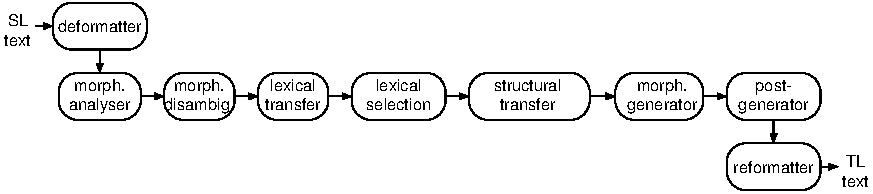
\includegraphics[width=0.8\textwidth]{architecture.pdf}
\end{center}
\caption{The pipeline architecture of the Apertium system.}
\label{fig:modules}
%\vspace{-1em}
\end{figure*}

The system is based on the Apertium machine translation 
platform \citep{apertium/2011}.\footnote{\url{http://www.apertium.org}} The 
platform was originally aimed at the Romance languages of the Iberian peninsula, but has also been adapted for 
other, more distantly related, language pairs.
The whole platform, both programs and data, are licensed under the Free Software Foundation's General Public 
Licence\footnote{\url{http://www.fsf.org/licensing/licenses/gpl.html}} (GPL) and all the software and data for the 
30 supported language pairs (and the other pairs being worked on) is available for download from the project 
website.

\subsection{Architecture of the system}

The Apertium translation engine consists of a Unix-style \emph{pipeline} or
\emph{assembly line} with the following modules (see Fig.~\ref{fig:modules}):  
\begin{itemise}
\item A \emph{deformatter} which encapsulates the format information
 in the input as \emph{superblanks} that will then be seen
 as blanks between words by the other modules.
\item A \emph{morphological analyser} which segments the text in
  surface forms (SF) (\emph{words}, or, where detected, multi-word lexical
  units or MWLUs) and for each, delivers one or more \emph{lexical
    forms} (LF) consisting of \emph{lemma}, \emph{lexical category} and
  morphological information. 
\item A \emph{morphological disambiguator} (constraint grammar) which chooses, using linguistic rules
  the most adequate sequence of morphological analyses for an ambiguous sentence. 
\item A \emph{lexical transfer} module which reads each SL LF 
  and delivers the corresponding target-language (TL) LF
  by looking it up in a bilingual dictionary encoded as an FST
  compiled from the corresponding XML file. The lexical transfer module may
  return more than one TL LF for a single SL LF.
\item A \emph{lexical selection} module which chooses, based on context 
  rules the most adequate translation of ambiguous source language LFs.
\item A \emph{structural transfer} module which
    performs local syntactic operations, is compiled from XML files containing rules that 
    associate an \emph{action} to each defined LF \emph{pattern}. Patterns are applied left-to-right, and the 
    longest matching pattern is always selected.
\item A \emph{morphological generator} which delivers a TL SF
 for each TL LF, by suitably inflecting it. 
\item A \emph{reformatter} which de-encapsulates any format
  information.
\end{itemise}


\subsection{Morphological transducers}

The morphological transducers are based on the Helsinki Finite State Toolkit \citep{hfst/2011}, a free/open-source reimplementation of the Xerox finite-state toolchain, popular in the field of morphological analysis. It implements both the \textbf{lexc} formalism for defining lexicons, and the \textbf{twol} and \textbf{xfst} formalisms for modeling morphophonological rules. It also supports other finite state transducer formalisms such as \textbf{sfst}. This toolkit has been chosen as it --- or the equivalent XFST --- has been widely used for other Turkic languages \citep{coltekin2010,altintas2001,tantug2006,washingtonipasovtyers12,tyerswashingtonsalimzyanbattalov12}, and is available under a free/open-source licence.

The morphologies of both languages are implemented in lexc, and the morphophonologies of both languages are implemented in twol.

Use of lexc allows for straightforward definition of different word classes and subclasses.  For example, Tatar (but not Kazakh) has two classes of verbs: one which takes a harmonised high vowel in the infinitive (the default), and one which take a harmonised low vowel in the infinitive.  This was implemented in lexc with two similar continuation lexica for verbs: one pointing at a lexicon with an A-initial infinitive ending, and another pointing at a lexicon with an I-initial infinitive ending.

Use of twol allows for phonological processes present in the languages, like vowel harmony and desonorisation, to be implemented in a straightforward manner.  For example, in Tatar, the A and I archiphonemes found in the infinitive are harmonised to one of two vowels each, depending on the value of the preceding vowel; the basic form of this process can be implemented in one twol rule.

The same morphological description is used for both analysis and generation. To avoid overgeneration, any alternative forms are 
marked with one of two marks, {\tt {\small LR}} (only analyser) or {\tt {\small RL}} (only generator). Instead of the usual
compile/invert to compile the transducers, we compile twice, once the generator, without the {\tt {\small LR}} paths, and
then again the analyser without the {\tt {\small RL}} paths. 

\subsection{Bilingual lexicon}
%FIXME: Ilnar, we need some good examples here
% ақпараттық құрал - мәгълүмат чарасы
% құрал - корал in other contexts

%<e>       <p><l>жай<s n="n"/></l>                 <r>җәя<s n="n"/></r></p></e> <!--"arch"-->
%<e>       <p><l>жай<s n="n"/></l>                 <r>урын<s n="n"/></r></p></e> <!--"place"-->
%<e>       <p><l>жай<s n="n"/></l>                 <r>хәл<s n="n"/></r></p></e> <!--"condition"-->
%<e>       <p><l>жай<s n="n"/></l>                 <r>яшен<s n="n"/></r></p></e> <!--"lightning"-->
	
\begin{figure*}[htbp]
\hspace{3cm}\parbox[t]{0.7\textwidth}{{\tt
%\begin{texttt}
    <e><p><l>\textbf{құрал}<s n="n"/></l><r>\textbf{корал}<s n="n"/></r></p></e> \\
    <e><p><l>\textbf{құрал}<s n="n"/></l><r>\textbf{чара}<s n="n"/></r></p></e> \\
    <e><p><l>\textbf{есім}<s n="n"/></l><r>\textbf{исем}<s n="n"/></r></p></e> \\
    <e><p><l>\textbf{топ}<s n="n"/></l><r>\textbf{туп}<s n="n"/></r></p></e> \\
    <e><p><l>\textbf{топ}<s n="n"/></l><r>\textbf{төркем}<s n="n"/></r></p></e> \\
    <e r="RL"><p><l>\textbf{топ}<s n="n"/></l><r>\textbf{группа}<s n="n"/></r></p></e>
}}%\end{texttt}
\caption{Example entries from the bilingual transfer lexicon. Kazakh is on the left, and Tatar on the right}
\label{fig:bidix}
%\vspace{-1em}
\end{figure*}

The bilingual lexicon currently contains 9,269 stem-to-stem correspondences and was built mostly 
by hand (i.e., by translating Kazakh stems unrecognised by the morphological analyser into Tatar).  Some 
toponyms and other proper names were translated semi-automatically by looking up links in Wikipedia \citep{tyers08}; also, 
some Russian loanwords common to both languages (such as автомобиль, гонорар, etc.) were added to the bilingual 
dictionary automatically by taking the intersection of Russian and Kazakh wordlists.

Entries consist largely of one-to-one stem-to-stem correspondences with part of speech, but also include some entries with ambiguous translations (see e.g., Fig.~\ref{fig:bidix}).

\subsection{Disambiguation rules}

The system has a morphological disambiguation module in the form of a 
Constraint Grammar (CG) \citep{karlsson95}. The version of the formalism used is vislcg3.\footnote{\url{http://beta.visl.sdu.dk/constraint_grammar.html}}

%FIXME: Describe the gist of the rules, maybe with a few concrete examples.
The grammar currently has 60 rules.  The goal of these rules is to select the correct analysis when there 
are multiple morphological analyses of Kazakh forms.
%FIXME: It might be good to put some numbers about the morphological ambiguity of Kazakh

%FIXME: JNW needs to copy-edit this, and we should probably provide a concrete example to make it clearer too
The output of the morphological analyser is highly ambiguous. Both Kazakh and Tatar have a lot of affixes which join the
verb stem. Some of the grammars label them all gerunds, or participles, assuming that there are no finite forms.

We give to a VerbStem+ParticularAffix surface form maximal number of readings (syntactic roles) it can have, such as [verbal
adjective], [finite form], [substantivised verbal adjective, i.e., if the word it determines was omitted], whereas many grammars
do not distinguish these and label forms of verbs containing a particular affix just as a certain gerund or participle form.

This type of ambiguity is common between the two languages we deal with, and therefore may be passed from one language
to another and most likely will not lead to translation errors. Disambiguating it, and, prior to that, having that kind of
informaton about the syntactical role of a surface form is crucial for success e.g. of a Turkic to English system. 

This is the reason for a high ambiguity rate of the transducers.
  
%but given the closeness of the languages, the 
%majority of ambiguity may be passed through from one language to the other.

\subsection{Lexical selection rules}

While many lexical items have a similar range of meaning, lexical selection can sometimes be problematic between Kazakh and Tatar.

For example (see figure~\ref{fig:bidix}), Kazakh құрал can mean an instrument, device, tool, or even weapon, all 
meanings corresponding to its Tatar cognate корал; however, it is also used in the 
compound ақпарат құралдары \eng{mass media} (literally, \eng{means of information}), which translates 
to Tatar as мәгълүмат чаралары (which has the same literal translation).  Hence, the Kazakh word құрал must have 
two entries in the bilingual lexicon: one that corresponds to Tatar корал and one that corresponds 
to Tatar чара.  A lexical selection rule that selects the translation чара when it occurs in a compound with ақпарат is written to ensure the correct translation; this rule is shown in figure~\ref{fig:lrx}.

\begin{figure*}[htbp]
\hspace{3cm}\parbox[t]{0.7\textwidth}{{\tt
%\begin{texttt}
  <rule> \\
    <match lemma="ақпарат" tags="n.attr"/> \\
    <match lemma="құрал" tags="n.*.px3sp.*"><select lemma="чара"/></match> \\
  </rule>
}}%\end{texttt}
\caption{A lexical selection rule that selects чара as the translation of құрал if part of a compound with ақпарат.}
\label{fig:lrx}
%\vspace{-1em}
\end{figure*}

Likewise, the Kazakh word топ has two translations into Tatar.  One translation is туп \eng{ball} (which can also 
be доп in Kazakh), and the other translation is төркем \eng{group}.  The bilingual dictionary also has 
the Russian word группа \eng{group}, which is used in Tatar, as an entry which may be translated 
to Kazakh топ (i.e., analysed), but is never generated.

The system currently has a total of 33 lexical selction rules.

%\subsection{Transfer rules}

\begin{table*}[htbp]
\centering
\begin{tabular}{ll}
%\hline
%{\bf Stage} & {\bf Representation} \\
\toprule
{\bf (Kazakh) Input} & Ол енді ол дыбысты анығырақ ести бастады. \\
%{\bf (Tatar) Input} & Һава бүген бик әйбәт, җылы гына. \\ 
\midrule
%{\bf Mor. analysis} & \^{}Һава/һава\tag{<n>}\tag{<attr>}/һава\tag{<n>}\tag{<nom>\$} \^{}бүген/бүген\tag{<adv>\$}  \\
% ~             & \^{}бик/бик\tag{<adv>}/бик\tag{<n>}\tag{<attr>}/бик\tag{<n>}\tag{<nom>\$} \\ 
% ~             & \^{}әйбәт/әйбәт\tag{<adj>}/әйбәт\tag{<adj>}\tag{<subst>}\tag{<nom>\$}\^{},/,\tag{<cm>\$} \\ 
% ~             & \^{}җылы/җылы\tag{<n>}\tag{<attr>}/җылы\tag{<n>}\tag{<nom>}/җылы\tag{<adj>}/җылы\tag{<adj>}\tag{<subst>}\tag{<nom>\$} \\
% ~             & \^{}гына/гына\tag{<postadv>\$}\^{}./.\tag{<sent>\$} \\
{\bf Mor.\ analysis} & \^{}Ол/ол\tag{<det>}\tag{<dem>}/ол\tag{<prn>}\tag{<dem>}\tag{<nom>}/\textbf{ол\tag{<prn>}\tag{<pers>}\tag{<p3>}\tag{<sg>}\tag{<nom>}}\tag{\$} \\
                     & \^{}енді/ен\tag{<n>}\tag{<acc>}/ен\tag{<v>}\tag{<iv>}\tag{<ifi>}\tag{<p3>}\tag{<pl>}/ен\tag{<v>}\tag{<iv>}\tag{<ifi>}\tag{<p3>}\tag{<sg>}/\textbf{енді\tag{<adv>}}\tag{\$}  \\
							& \^{}ол/\textbf{ол\tag{<det>}\tag{<dem>}}/ол\tag{<prn>}\tag{<dem>}\tag{<nom>}/ол\tag{<prn>}\tag{<pers>}\tag{<p3>}\tag{<sg>}\tag{<nom>}\tag{\$} \\
                     & \^{}дыбысты/\textbf{дыбыс\tag{<n>}\tag{<acc>}}\tag{\$} \\
							& \^{}анығырақ/анық\tag{<adj>}\tag{<comp>}/\textbf{анық\tag{<adj>}\tag{<comp>}\tag{<advl>}}/анық\tag{<adj>}\tag{<comp>}\tag{<subst>}\tag{<nom>}\tag{\$} \\
                     & \^{}ести/\textbf{есті\tag{<v>}\tag{<tv>}\tag{<prc\_impf>}}\tag{\$}  \\
                     & \^{}бастады/баста\tag{<v>}\tag{<tv>}\tag{<ifi>}\tag{<p3>}\tag{<pl>}/баста\tag{<v>}\tag{<tv>}\tag{<ifi>}\tag{<p3>}\tag{<sg>}/баста\tag{<vaux>}\tag{<ifi>}\tag{<p3>}\tag{<pl>} \\
                     & \hspace{2em}/\textbf{баста\tag{<vaux>}\tag{<ifi>}\tag{<p3>}\tag{<sg>}}\tag{\$}  \\
\midrule
%{\bf Mor. disambiguation}& \^{}Һава\tag{<n>}\tag{<nom>\$} \^{}бүген\tag{<adv>\$} \^{}бик\tag{<adv>\$} \^{}әйбәт\tag{<adj>\$}\^{},\tag{<cm>\$} \\ 
{\bf Mor.\ disambiguation} & \^{}Ол\tag{<prn>}\tag{<pers>}\tag{<p3>}\tag{<sg>}\tag{<nom>}\tag{\$} \^{}енді\tag{<adv>}\tag{\$} \^{}ол\tag{<det>}\tag{<dem>}\tag{\$} \^{}дыбыс\tag{<n>}\tag{<acc>}\tag{\$} \\
                     & \^{}анық\tag{<adj>}\tag{<comp>}\tag{<advl>}\tag{\$} \^{}есті\tag{<v>}\tag{<tv>}\tag{<prc\_impf>}\tag{\$} \^{}баста\tag{<vaux>}\tag{<ifi>}\tag{<p3>}\tag{<sg>}\tag{\$}\^{}.\tag{<sent>}\tag{\$} \\
\midrule
{\bf Lex. transfer} & \^{}Ол\tag{<prn>}\tag{<pers>}\tag{<p3>}\tag{<nom>}/Ул\tag{<prn>}\tag{<pers>}\tag{<p3>}\tag{<nom>}\tag{\$} \^{}енді\tag{<adv>}/инде\tag{<adv>}/хәзер\tag{<adv>}\tag{\$} \\
 ( + selection)     & \^{}ол\tag{<det>}\tag{<dem>}/ул\tag{<det>}\tag{<dem>}\tag{\$} \^{}дыбыс\tag{<n>}\tag{<acc>}/тавыш\tag{<n>}\tag{<acc>}\tag{\$} \\
                    & \^{}анық\tag{<adj>}\tag{<comp>}\tag{<advl>}/анык\tag{<adj>}\tag{<comp>}\tag{<advl>}\tag{\$}  \\
						  & \^{}есті\tag{<v>}\tag{<tv>}<prc\_impf>/ишет\tag{<v>}\tag{<tv>}\tag{<prc\_impf>}\tag{\$} \\
                    & \^{}баста\tag{<vaux>}\tag{<ifi>}\tag{<p3>}\tag{<sg>}/башла\tag{<vaux>}\tag{<ifi>}\tag{<p3>}\tag{<sg>}\tag{\$}\^{}.\tag{<sent>}/.\tag{<sent>}\tag{\$} \\
%\^{}Һава\tag{<n>}\tag{<nom>}/Һауа\tag{<n>}\tag{<nom>\$} \^{}бүген\tag{<adv>}/бөгөн\tag{<adv>\$} \^{}бик\tag{<adv>}/бик\tag{<adv>\$} \\
%                     & \^{}әйбәт\tag{<adj>}/әйбәт\tag{<adj>\$}\^{},\tag{<cm>}/,\tag{<cm>\$} \^{}җылы\tag{<adj>}/йылы\tag{<adj>\$} \\ 
%~                     & \^{}гына\tag{<postadv>}/ғына\tag{<postadv>\$}\^{}.\tag{<sent>}/.\tag{<sent>\$}\\
\midrule
{\bf Struct. transfer}& \^{}Ул\tag{<prn>}\tag{<pers>}\tag{<p3>}\tag{<nom>}\tag{\$} \^{}инде\tag{<adv>}\tag{\$} \^{}ул\tag{<det>}\tag{<dem>}\tag{\$} \^{}тавыш\tag{<n>}\tag{<acc>}\tag{\$} \\
                      & \^{}анык\tag{<adj>}\tag{<comp>}\tag{<advl>}\tag{\$} \^{}ишет\tag{<v>}\tag{<tv>}\tag{<prc\_impf>}\tag{\$} \^{}башла\tag{<vaux>}\tag{<ifi>}\tag{<p3>}\tag{<sg>}\tag{\$}\^{}.\tag{<sent>}\tag{\$} \\

%\^{}Һауа\tag{<n>}\tag{<nom>\$} \^{}бөгөн\tag{<adv>\$} \^{}бик\tag{<adv>\$} \^{}әйбәт\tag{<adj>\$}\^{},\tag{<cm>\$} \\ 
%~                    & \^{}йылы\tag{<adj>\$} \^{}ғына\tag{<postadv>\$}\^{}.\tag{<sent>\$}\\
\midrule
{\bf Mor. generation} & Ул инде ул тавышны аныграк ишетә башлады. \\
\bottomrule
\end{tabular}
 \caption{Translation process for the Kazakh phrase \emph{Ол енді ол дыбысты анығырақ ести бастады} \eng{He begins to listen to that sound more carefully}.}
 %\vspace{-1em}
\end{table*}

\section{Evaluation}
\label{sec:eval}

Lexical coverage of the system is calculated over freely available corpora of Kazakh and Tatar.

For Kazakh, two years worth of content (2010 and 2012) from Radio Free Europe / Radio Liberty's Kazakh-language service,\footnote{\url{http://www.azattyq.org/}} as well as a recent dump of Wikipedia's articles in Kazakh\footnote{\url{http://kk.wikipedia.org/}; {\smallertt kkwiki-20130408-pages-articles.xml.bz2}} were used.

For Tatar, the Tatar Wikipedia,\footnote{\url{http://tt.wikipedia.org/}; {\smallertt ttwiki-20130205-pages-articles.xml.bz2}} the New Testament in Tatar, and content from Radio Free Europe / Radio Liberty's Tatar-language service\footnote{\url{http://www.azatlyk.org/}} from early 2007 to early 2012.

%The versions of the transducers tested were {\tt {\small r43595}} from the Apertium SVN.\footnote{\url{https://apertium.svn.sourceforge.net/svnroot/apertium}}  Corpora were divided into 10 parts each; the coverage numbers given are the averages of the calculated percentages of number of words analysed for each of these parts, and the standard deviation presented is the standard deviation of the coverage on each corpus.

%%
%%\begin{table}[htbp]
%%	\centering
%%	\subfloat[Coverage of Kazakh transducer over Kazakh corpora]{
%%		\begin{tabular}{llrrr}
%%			\toprule
%%			Corpus          & Tokens & Coverage & stdev\\
%%			\midrule
%%			RFERL 2010      & 3.2M   & 90.26\% & 0.24\% \\
%%			RFERL 2012      & 2.9M   & 89.81\% & 0.59\% \\
%%			Wikipedia       & 1.2M   & 80.56\% & 5.44\% \\
%%			\bottomrule
%%		\end{tabular}
%%	}\\
%%	\subfloat[Coverage of Tatar transducer over Tatar corpora]{
%%		\begin{tabular}{llrrr}
%%			\toprule
%%			Corpus          & Tokens & Coverage & stdev\\
%%			\midrule
%%			RFERL 2007-2012 & 1.2M   & 82.56\%  & 3.24\% \\
%%			Wikipedia       & 128K   & 82.23\%  & 1.58\% \\
%%			New Testament   & 137K   & 92.54\%  & 1.31\% \\
%%			\bottomrule
%%		\end{tabular}
%%	}
%%	\caption{Naïve vocabulary coverage of the stand-alone transducers.}
%%	\label{table:coverage}
%%\end{table}


\begin{table}
	\centering
	\subfloat[Naïve coverage of the Kazakh-Tatar direction]{
		\begin{tabular}{llrrr}
			\toprule
			Corpus          & Tokens & Coverage & stdev\\
			\midrule
			RFERL 2010      & 3.2M   & 90.19\% & $\pm$ 0.23\% \\
			RFERL 2012      & 2.9M   & 89.74\% & $\pm$ 0.59\% \\
			Wikipedia       & 1.2M   & 80.75\% & $\pm$ 5.23\% \\
			\bottomrule
		\end{tabular}
	}\\
	\subfloat[Naïve coverage of the Tatar-Kazakh direction]{
		\begin{tabular}{llrrr}
			\toprule
			Corpus          & Tokens & Coverage & stdev\\
			\midrule
			RFERL 2007-2012 & 1.2M   & 82.24\% & $\pm$ 2.88\% \\
			New Testament   & 137K   & 91.79\% & $\pm$ 1.39\% \\
			Wikipedia       & 128K   & 81.36\% & $\pm$ 1.48\% \\
			\bottomrule
		\end{tabular}
	}

	\caption{Naïve coverage of the Kazakh-Tatar system}
	\label{table:trimmedcoverage}
\end{table}

As shown in table~\ref{table:trimmedcoverage}, the naïve coverage of the Kazakh-Tatar MT 
system\footnote{Note that the coverage of the vanilla transducers is somewhat higher.} over 
the news corpora approaches that of a broad-coverage MT system, with one word in ten unknown.
For the Wikipedia corpus, the coverage 
is substantially worse.  This is due to the fact that this corpus is ``dirtier'' --- 
containing more orthographical errors, \emph{wiki} code, and repetitions, as well as to the 
fact that it has contains many more proper nouns.

To measure the performance of the translator we used the Word Error Rate metric --- an edit-distance metric based on the
Levenshtein distance \citep{levenshtein/1966}.

We had two small Kazakh corpora along with their postedited translations into Tatar to measure the WER.
The first one (2,457 words total) was a concatenation of an article from Radio Free Europe / Radio Liberty's
Kazakh-language service, an article from Wikipedia, and a simple story used for pedagogical purposes in a workshop
on MT for the languages of Russia. In addition to postediting the translation, this corpus was run through the
morphological transducer and its output was manually disambiguated. All the stems in these texts had been added to
the system, and all the rules (Constraint Grammar, lexical selection and transfer) were based on this corpus.
Hence we can call it the development corpus. It presents an upper bound on the current performance
of the system. Table~\ref{table:wer-development} presents the WER for it. % http://pastebin.com/TaaWxJzN

The second corpus --- a collection of articles from Radio Free Europe / Radio Liberty's Kazakh-language service --- was used solely for evaluation.  It had a similar size --- 2,862 words.
The WER results for this corpus are presented in table~\ref{table:wer-development}. % http://pastebin.com/7tzGCgMX.

Some of the corrections that were made as part of postediting were due the lack of morphophonoligical rules in the Tatar transducer, and were not translation errors as such.

\todo{Example of lack of phon rule}

%The WER on the translation of the development corpus and its postedited version is twice as low.
%Which, considering the relatively low number of rules, indicates that a high quality translation can be achived
%by advancing these two modules.

%To get an idea of the kind of performance that could be expected from the system, we 
%translated a simple story from Tatar to Bashkir and vice versa. The story may be found 
%online,\footnote{\url{https://apertium.svn.sourceforge.net/svnroot/apertium/branches/xupaixkar/rasskaz}}
%and was used for pedagogical purposes in a recently workshop on MT
%for the languages of Russia.

\begin{table}
  \begin{center}
  \begin{tabular}{ccrrr}
  \toprule
   Corpus                 & Direction           & Tokens  & OOV & WER (\%) \\
  \midrule
  \texttt{devel} & kaz$\rightarrow$tat & 2457    & 2       & 15.19 \\
  \bottomrule
  \texttt{test} & kaz$\rightarrow$tat & 2862    & 43      & 36.57 \\
  \end{tabular}
    \caption{Word error rate over two corpora. The \texttt{devel} `development' corpus was used during development 
       to identify possible disambiguation, lexical-selection and transfer rules. The \texttt{test} corpus
       was not seen during development. The OOV column gives the number of out-of-vocabulary (unknown) words.}
 %\vspace{-2.5em}
    \label{table:wer-development}
  \end{center}
\end{table}

%Table~\ref{table:wer} presents the Word Error Rate, an edit metric based on the Levenshtein 
%distance \citep{levenshtein/1966}. This measure was calculated once all the stems in the 
%text had been added to the system, thus presents an upper bound on the current performance
%of the transfer lexicon, and the disambiguation and transfer rules.

%We calculate the WER instead of other MT evaluation metrics such as BLEU as the WER is 
%geared towards a particular task, that of measuring postedition effort. The translations 
%of the story into Tatar and Bashkir were done in parallel to make them as close as possible,
%so using BLEU would give an over-optimistic view of the quality.

\subsection{Error analysis}

%The majority of errors are currently due to mistakes and gaps in the morphophonology component; some minor problems still remain involving:
%\begin{itemise}
%  \item Combinations of case and possessive suffixes,
%  \item Orthographical representations of phonology,
%  \item Vowel harmony processing on clitics (e.g., \emph{да}/\emph{дә} `and') after unknown words.
%\end{itemise}

%\cite{TyersAlperen2010}

%challenges:

%% making bidirectional systems
%% when the morphotactics does not line up

\section{Concluding remarks}
\label{sec:conc}

To our knowledge we have presented the first ever MT system between Kazakh and Tatar. It has a near-to-production-level
coverage, but rather a prototype-level number of rules. Though the impact of this relatively low number of rules on the
quality of the translation (compare the WER results for the corpus 1 and corpus 2) looks very promising and suggests
the a high-quality translation between morphologically-rich agglutinative languages is possible.

We plan to continue development on the pair; the coverage of the system is already quite high, and although we intend to
increase it to 95\% on the corpora we have, the main work will be improving the quality of the translation by adding
more rules, starting with the Constraint Grammar module.
The long-term plan is to integrate the data created with other open-source data for Turkic languages in order to make
transfer systems between all the Turkic language pairs.  Related work is currently ongoing with Chuvash--Turkish and Turkish--Kyrgyz.

The system is available as free/open-source software under the GNU GPL and the whole system may be downloaded
from SVN.\footnote{\url{https://apertium.svn.sourceforge.net/svnroot/apertium/staging/apertium-kaz-tat}}

\section*{Acknowledgements}

The work on this Kazakh-Tatar machine translation system was partially funded by the Google Summer of Code and Google Code-In programmes.

%\bibliographystyle{lrec2012}
%\bibliography{tt-ba}
\bibliographystyle{mtsxiv}
%\bibliographystyle{apa}
\bibliography{paper}

\end{document}
